\documentclass[../Homework]{subfiles}

\begin{document}
	\section{Chi-Square Tests for Goodness of Fit}
		\paragraph{1. Aw, nuts!}
			\begin{enumerate}[a.]
				\item
					\begin{align*}
						H_0&: \text{The true distribution of mixed nuts is just as the company claims.} \\
						H_a&: \text{The true distribution of mixed nuts differs from what the company claims.}
					\end{align*}
				\item
					\begin{align*}
						\text{Cashew} &= 0.52(150) = 78 = 78 & \text{Almond} &= 0.27(150) = 40.5 \\
						\text{Macadamia} &= 0.13(150) = 19.5 & \text{Brazil} &= 0.08(150) = 12
					\end{align*}
			\end{enumerate}
				\[\chi^2 = \sum\left[\mathrm{\frac{(observed - expected)^2}{expected}}\right] \approx 6.599\]
		\paragraph{3. $P$-values}
			\begin{enumerate}
				\item
					\begin{align*}
						0.05 < \pval &< 0.1 \\
						\pval &= \chiCDF{19.03}{\infty}{11} \approx 0.061
					\end{align*}
				\item
					\begin{align*}
						\pval &< 0.0005 \\
						\pval &= \chiCDF{19.03}{\infty}{3} \approx 2.695 \times 10^{-4}
					\end{align*}
			\end{enumerate}
		\paragraph{5. Aw, nuts!}
			\begin{enumerate}[a.]
				\item
					There are over 5 counts expected in each category, so the Large Counts condition is met.
					\[\df = \text{categories} - 1 = 4 - 1 = 3\]
				\item
					\begin{align*}
						0.05 < \pval &< 0.1 \\
						\pval &= \chiCDF{\chi^2 \approx 6.599}{\infty}{n - 1 = 4 - 1 = 3} \approx 0.086
					\end{align*}
				\item
					Over many trials, there is an 8.6\% probability of receiving a difference at at least as great as that observed from the claimed proportions.
				\item
					As the $\pval$ of about 8.6\% is greater than the significance level $\alpha = 0.05$, the null hypothesis cannot be rejected. The data does not provide convincing evidence that the true proportions of deluxe mixed nuts significantly differ from those claimed.
			\end{enumerate}
		\paragraph{9. Munching Froot Loops}
			\begin{align*}
				H_0&: \text{The proportions of Froot Loop colors are those claimed by Kellogg's.} \\
				H_a&: \text{The proportions of Froot Loop colors are not those claimed by Kellogg's.}
			\end{align*}
			The sample was random, so the Randomness condition is met. \\
			There are over 1200 Froot Loops, so the sample size of 120 is less than 10\% of the population size. \\
			As the probabilities are equal, the expected counts of each color is equal, being $120/6 = 20$. \\
			As the expected counts of all categories is 20, which is greater than 5, the Large Counts condition is met. \\
			\begin{align*}
				\chi^2 &= \sum\left[\mathrm{\frac{(observed - expected)^2}{expected}}\right] = 7.9 \\
				\df &= \text{categories} - 1 = 6 - 1 = 5 \\
				\pval &= \chiCDF{7.9}{\infty}{5} \approx 0.162
			\end{align*}
			As the $\pval$ of about 0.162 is greater than the significance level of $\alpha = 0.05$, the null hypothesis cannot be rejected. The data does not provide convincing evidence that the true proportions of Froot Loops colors differs from those claimed by Kellogg's.
		\paragraph{13. Birds in the tress}
			\begin{enumerate}[a.]
				\item
					\begin{align*}
						H_0&: \text{The red-breasted nuthatches have no preference regarding trees.} \\
						H_a&: \text{The red-breasted nuthatches have some preference regarding trees.}
					\end{align*}
					The sample was random, so the Randomness condition is met. \\
					The sample size of 156 is likely less than 10\% of the number of red-breasted nuthatches in the forest, so the 10\% condition is met, justifying independence. \\
					\begin{align*}
						\text{Douglas firs} &= (0.54)(312) = 84.24 & \text{ponderosa pines} &= (0.4)(156) = 62.4 \\
						\text{other} &= (0.06)(156) = 9.36
					\end{align*}
					The expected counts of each category are greater than 5, so the Large Counts condition is met. \\
					\begin{align*}
						\chi^2 &= \sum\left[\mathrm{\frac{(observed - expected)^2}{expected}}\right] \approx 7.418 \\
						\df &= \text{categories} - 1 = 3 - 1 = 2 \\
						\pval &= \chiCDF{\chi^2 \approx 7.418}{\infty}{2} \approx 0.024 
					\end{align*} \\
					As the $\pval$ of about 0.024 is less than the significance level $\alpha = 0.05$, the null hypothesis can be rejected. The data provides convincing evidence that red-breasted nuthatches have some preference regarding trees.
				\item
					\[\begin{array}{|c|c|c|c|}\hline
						\text{tree} & \text{observed} & \text{expected} & \mathrm{observed - expected} \\\hline
						\text{Douglas firs} & 70 & 84.24 & -14.24 \\\hline
						\text{ponderosa pines} & 79 & 62.4  & 16.6 \\\hline
						\text{other} & 7 & 9.36 & -2.36 \\\hline
					\end{array}\]
					The greatest (and only) positive difference between the observed and expected counts indicates that red-breasted nuthatches prefer ponderosa pines. The greatest negative difference indicates that they are most averse to Douglas firs.
			\end{enumerate}
		\paragraph{15. Mendel and the peas}
			\begin{enumerate}[a.]
				\item
					\begin{align*}
						H_0&: \text{The actual proportions of smooth and wrinkled peas are 0.75 and 0.25 respectively.} \\
						H_a&: \text{The actual proportions of smooth and wrinkled peas are not \(0.75\) and \(0.25\) respectively}
					\end{align*}
					\[\begin{array}{|c|c|c|}\hline
						& \text{observed} & \text{expected} \\\hline
						\text{smooth} & 423 & 0.75(423 + 133) = 417 \\\hline
						\text{wrinkled} & 133 & 0.25(423 + 133) = 139 \\\hline
					\end{array}\]
					\begin{align*}
						\chi^2 &= \sum\left[\mathrm{\frac{(observed - expected)^2}{expected}}\right] \approx 0.345 \\
						\df &= \text{categories} - 1 = 2 - 1 = 1 \\
						\pval &= \tCDF{\chi^2 \approx 0.345}{\infty}{1} \approx 0.557
					\end{align*}
					As the $\pval$ of about 0.557 is greater than the significance level $\alpha = 0.05$, the null hypothesis cannot be rejected. The data does not provide convincing evidence that the true proportions of smooth and wrinkled peas are not 0.75 and 0.25 respectively.
				\item
					\begin{align*}
						\hat{p} &= \frac{423}{423 + 133} \approx 0.761 \\
						s_{\hat{p}} &= \propse{\hat{p}}{n} \approx \propse{0.761}{423 + 133} \approx 0.018 \\ 
						z &= \z{\hat{p}}{p_0}{s_{\hat{p}}} \approx \z{0.761}{0.75}{0.018} \approx 0.596 \\
						\pval &= 1 - \normalCDF{-z \approx -0.596}{z \approx 0.596}{0}{1} \approx 0.551
					\end{align*}
					As the $\pval$ of about 0.551 is greater than the significance level $\alpha = 0.05$, the null hypothesis cannot be rejected. The data does not provide convincing evidence that the true proportion smooth peas is not equal to 0.75.
			\end{enumerate}
		\paragraph{17. Is your random number generator working?}
			\begin{enumerate}[a.]
				\item
					\begin{align*}
						H_0&: \text{Each digit's proportion is 0.1.} & H_a&: \text{Not every digit's proportion is 0.1}
					\end{align*}
					The randomness condition is met, as the numbers were randomly generated. \\
					The independence condition is met, as each digit being generated was independent of the last. \\
					\[\begin{array}{|c|c|c|c|c|c|c|c|c|c|c|}\hline
						\text{digit} & 0 & 1 & 2 & 3 & 3 & 5 & 6 & 7 & 8 & 9 \\\hline
						\text{observed} & 18 & 20 & 25 & 25 & 21 & 15 & 18 & 19 & 13 & 26 \\\hline
						\text{expected} & 0.1(200) = 20 & 20 & 20 & 20 & 20 & 20 & 20 & 20 & 20 & 20 \\\hline
					\end{array}\]
					The Large Counts condition is met, as each digit is expected to be generated 20 times, which is greater than 5.
				\item
					\begin{align*}
						\chi^2 &= \sum\left[\mathrm{\frac{(observed - expected)^2}{expected}}\right] = 6.7 \\
						\df &= \text{categories} - 1 = 10 - 1 = 9 \\
						\pval &= \chiCDF{\chi^2 = 6.7}{\infty}{9} \approx 0.668
					\end{align*}
					As the $\pval$ of 0.668 is greater than the significance level $\alpha = 0.05$, the null hypothesis cannot be rejected. The data does not provide convincing evidence of the true proportions of randomly generated digits being nonuniform. \\
				\item
					The probability of a Type \Roman{1} error occurring is equal to the significance level $\alpha = 0.05$. \\
				\item
					The probability of a Type \Roman{1} error occurring is the same for every trial. \\
					The number of trials is fixed at 25. \\
					A Type \Roman{1} error can either occur or not occur, making the outcome binary. \\
					The number of Type \Roman{1} errors is therefore a binomial variable.
					\[P(X \ge 1) = 1 - P(X = 0) = 1 - \binom{25}{0}(0.05)^0(1 - 0.05)^{25 - 0} \approx 0.277\]
			\end{enumerate}
		\paragraph{19.}\ \\
			The null hypothesis should describe population proportions, making the answer \textbf{d}.
		\paragraph{20.}
			\[\chi^2 = \sum\left[\mathrm{\frac{(observed - expected)^2}{expected}}\right]\]
			The answer is therefore \textbf{a}.
		\paragraph{21.}\ \\
			A $\pval$ less than the significance level results in $H_0$ being rejected due to the data providing convincing evidence for $H_a$. The answer is therefore \textbf{c}.
		\paragraph{22.}\ \\
			The degrees of freedom for a chi-square test is determined by the number of categories, not the sample size. The answer is therefore \textbf{c}.
		\paragraph{23. Video games}
			\begin{enumerate}[a.]
				\item\
					\begin{center}
						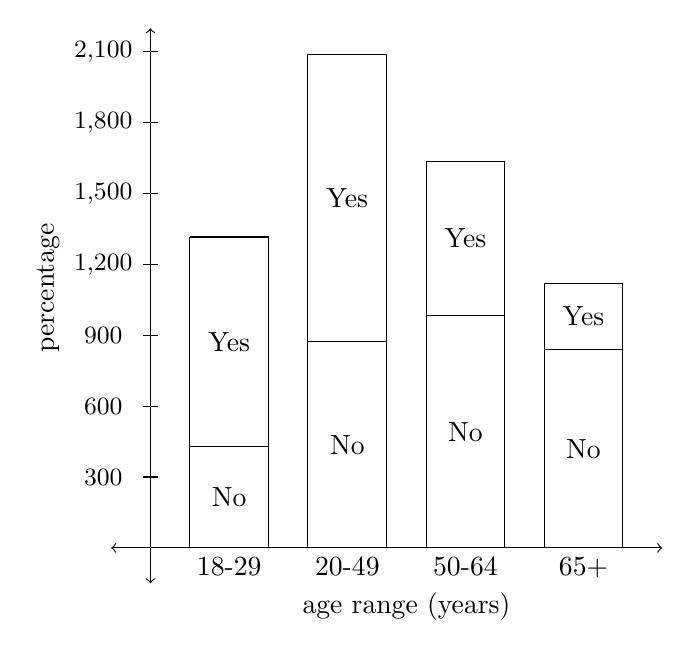
\begin{tikzpicture}[yscale = 3]
							%Axes
							%TODO Fix (standardize)
							\draw[<->] (-0.5, 0) -- (6.5, 0);
								\node[] at (6.5/2, -0.25) {age range (years)};
							\draw[<->] (0, -0.15) -- (0, 2.2);
								\node[rotate = 90] at (-1.3, 2.2/2) {percentage};
							\foreach \x in {1,...,7}
								\draw[] (-0.1, \x * 0.3) -- (0.1, \x * 0.3);
							\foreach \x in {1,...,7}
								\pgfmathparse{\x * 300} \pgfmathprintnumberto{\pgfmathresult}\fx
								\node at (-0.6, \x * 0.3) {\small \fx};
							%Columns
							 	%18-29
								\draw[] (0.5, 0) -- (0.5, 1.316);
								\draw[] (1.5, 0) -- (1.5, 1.316);
								\draw[] (0.5, 1.316) -- (1.5, 1.316);
								\draw[] (0.5, 0.429) -- (1.5, 0.429);
								\node[below] at (1, 0) {18-29};
								\node[] at (1, 0.429/2) {No};
								\node[] at (1, 0.887/2 + 0.429) {Yes};
								%30-49
								\draw[] (2, 0) -- (2, 2.089);
								\draw[] (3, 0) -- (3, 2.089);
								\draw[] (2, 2.089) -- (3, 2.089);
								\draw[] (2, 0.872) -- (3, 0.872);
								\node[below] at (2.5, 0) {20-49};
								\node[] at (2.5, 0.872/2) {No};
								\node[] at (2.5, 1.217/2 + 0.872) {Yes};
								%60-64
								\draw[] (3.5, 0) -- (3.5, 1.635);
								\draw[] (4.5, 0) -- (4.5, 1.635);
								\draw[] (3.5, 1.635) -- (4.5, 1.635);
								\draw[] (3.5, 0.985) -- (4.5, 0.985);
								\node[below] at (4, 0) {50-64};
								\node[] at (4, 0.985/2) {No};
								\node[] at (4, 0.65/2 + 0.985) {Yes};
								%65+
								\draw[] (5, 0) -- (5, 1.119);
								\draw[] (6, 0) -- (6, 1.119);
								\draw[] (5, 1.119) -- (6, 1.119);
								\draw[] (5, 0.84) -- (6, 0.84);
								\node[below] at (5.5, 0) {65+};
								\node[] at (5.5, 0.84/2) {No};
								\node[] at (5.5, 0.279/2 + 0.84) {Yes};
						\end{tikzpicture}
					\end{center}
				\item
					The lower the age, the higher the proportion of people that play video games.
			\end{enumerate}
	\section{Inference for Two-Way Tables}
		\paragraph{27. The color of candy}\ \\
			Those that took a colored survey showed a strong preference for the candy of the same color while those in the control group slightly preferred the blue candy.
		\paragraph{29. More candy}
			\begin{enumerate}[a.]
				\item		
					\begin{align*}
						H_0&: \text{The distributions of candy colors remains the same regardless of the survey.} \\
						H_a&: \text{The distributions of candy colors is affected by the survey.}
					\end{align*}
				\item
					\[\begin{tabular}{|c|c|c|}\hline
						& Red & Blue \\\hline
						Red & $\frac{20(26)}{60} = 8.\overline{3}$ & $\frac{20(26)}{60} = 8.\overline{3}$ \\\hline
						Blue & $\frac{20(34)}{60} = 11.\overline{3}$ & $\frac{20(34)}{60} = 11.\overline{3}$ \\\hline
					\end{tabular}\]
				\item
					\[\chi^2 = \sum\left[\mathrm{\frac{(observed - expected)^2}{expected}}\right] \approx 6.652\]
			\end{enumerate}			
		\paragraph{31. Last candy}
			\begin{enumerate}[a.]
				\item
					The Randomness condition is met, as the assignment was random. \\
					The independence condition is met, as this is an experiment. \\
					The Large Counts condition is met, as all expected values are greater than 5.
				\item
					\begin{align*}
						0.005 < \pval &< 0.01 \\
						\pval &= \tCDF{\chi^2 \approx 6.652}{\infty}{(2 - 1)(3 - 1) = 2} \approx 0.036
					\end{align*}
				\item
					If the survey has no affect on preferences, the probability of receiving data that differ from the expected values at least as much as those observed is about 3.6\%.
				\item
					As the $\pval$ of about 0.036 is greater than the significance level $\alpha = 0.01$, the null hypothesis cannot be rejected. The data does not provide convincing evidence that the survey affects the preferences for candy color.
			\end{enumerate}
		\paragraph{33. Sorry, no chi-square}\ \\
			The counts of the travelers from each category is not known, just the relative frequencies of each category.
		\paragraph{34. Going nuts}\ \\
			The data describes means rather than counts (proportions).
		\paragraph{35. Gummy bears}
			\begin{align*}
				H_0&: \text{The distributions of colors is the same for name and store-brand gummy bears} \\
				H_a&: \text{The distributions of colors differs for name and store-brand gummy bears}
			\end{align*}
			The randomness condition is met, as the samples were random. \\
			The independence condition is met, as there are over 6 bags is far less than 10\% of the number of bags of name or store-brand gummy bears. \\
			\[\begin{tabular}{|c|c|c|}\hline
				& Name & Store \\\hline
				Red & 130.83 & 218.17 \\\hline
				Green & 58.86 & 98.15 \\\hline
				Yellow & 50.61 & 84.39 \\\hline
				Orange & 77.97 & 130.03 \\\hline
				White & 54.742 & 91.268 \\\hline
			\end{tabular}\]
			Every expected count exceeds 5, so the Large Counts condition is met.
			\begin{align*}
				\chi^2 &= \sum\left[\mathrm{\frac{(observed - expected)^2}{expected}}\right] \approx 1.815 \\
				\df &= (2 - 1)(5 - 1) = 4 \\
				\pval &= \chiCDF{\chi^2 \approx 1.815}{\infty}{4} \approx 0.77
			\end{align*}
			As the $\pval$ of about 0.77 is greater than the significance level $\alpha = 0.05$, the null hypothesis cannot be rejected. The data does not provide convincing evidence of a difference existing between the true distributions of gummy bear colors for name and store brands.
		\paragraph{37. How to quit smoking}
			\begin{enumerate}[a.]
				\item
					\[\begin{tabular}{|c|c|c|c|c|c|}\hline
						& Nicotine patch & Drug & Patch plus drug & Placebo & Total \\\hline
						Successes & 40 & 74 & 87 & 25 & 226  \\\hline
						Failures & 204 & 170 & 158 & 135 & 667 \\\hline
						Total & 244 & 244 & 245 & 160 & 893 \\\hline
					\end{tabular}\]
				\item
					\begin{align*}
						H_0&: \text{The proportions of successes and failures is the same across all treatments.} \\
						H_a&: \text{The proportions of successes and failures is not the same across all treatments.}
					\end{align*}
					The randomness condition is met, as the assignment was random. \\
					The independence condition is met, as this is an experiment. \\
					\[\begin{tabular}{|c|c|c|c|c|}\hline
						& Nicotine patch & Drug & Patch plus drug & Placebo \\\hline
						Successes & 61.75 & 61.75 & 62 & 40.49 \\\hline
						Failures & 182.25 & 182.25 & 183 & 119.51 \\\hline
					\end{tabular}\]
					Every expected count is greater than 5, so the Large Counts condition is met.
					\begin{align*}
						\chi^2 &= \sum\left[\mathrm{\frac{(observed - expected)^2}{expected}}\right] \approx 34.937 \\
						\df &= (4 - 1)(2 - 1) = 3 \\
						\pval &= \chiCDF{\chi^2 \approx 34.937}{\infty}{3} \approx 1.256 \times 10^{-7}
					\end{align*}
					As the $\pval$ of about $1.256 \times 10^{-7}$ is less than the significance level $\alpha = 0.05$, the null hypothesis can be rejected. The data provides convincing evidence that different treatments result in a different distribution of successes and failures.
			\end{enumerate}
		\paragraph{39. How to quit smoking}\ \\
			The treatment with the largest positive difference between its actual and expected values is the combination of the patch and drug, suggesting that is is the most effective. The one with the largest negative difference, on the other hand, is the nicotine patch, indicating that it is the least effective treatment.
		\paragraph{41. Relaxing in the sauna}
			\begin{enumerate}[a.]
				\item
					\begin{align*}
						H_0&: \text{The distribution of suffering from SCD is independent of weekly sauna frequency.} \\
						H_a&: \text{Weekly sauna frequency affects the distribution of suffering from SCD.}
					\end{align*}
				\item
					\[\begin{tabular}{|c|c|c|c|}\hline
						& <1 & 2-3 & >4 \\\hline
						Yes & 49.33 & 124.18 & 17.5 \\\hline
						No & 551.67 & 1388.8 & 184.5 \\\hline
					\end{tabular}\]
				\item
					\begin{align*}
						\chi^2 &= \sum\left[\mathrm{\frac{(observed - expected)^2}{expected}}\right] \approx 6.032 \\
						\df &= (3 - 1)(2 - 1) = 2 \\
						\pval &= \chiCDF{\chi^2 \approx 6.032}{\infty}{2} \approx 0.049
					\end{align*}
				\item
					As the $\pval$ of about 0.049 is less than the significance level $\alpha = 0.05$, the null hypothesis can be rejected. The data provides convincing evidence that going to the sauna affects the distribution of SCD suffering.
			\end{enumerate}
		\paragraph{43. Finger length}
			\begin{align*}
				H_0&:
			\end{align*}
		\paragraph{47.}
		\paragraph{53.}
		\paragraph{65.}
		\paragraph{66.}
		\paragraph{67.}
		\paragraph{68.}
	\section{Inference for Slopes}
		\paragraph{69.}
		\paragraph{71.}
		\paragraph{73.}
		\paragraph{25.}
		\paragraph{77.}
		\paragraph{79.}
		\paragraph{83.}
		\paragraph{85.}
		\paragraph{87.}
		\paragraph{88.}
		\paragraph{89.}
		\paragraph{91.}
		\paragraph{92.}
\end{document}